\chapter{Ma collaboration au projet}\label{collab}
\putminitoc
Après avoir défini plus en détails les besoins de notre plateforme et son fonctionnement général, nous allons maintenant voir en détail de quelle manière j'ai contribué à ce projet. En parallèle de la maintenance de notre plateforme, j'ai développé deux nouvelles fonctionnalités. Ces deux fonctionnalités ayant un rapport direct avec la notion de << calibration >>, nous allons tout d'abord définir celles-ci avant de voir en détail mon développement et la maintenance que j'ai effectué.

\section{Les calibrations}
Une calibration est une constante stockée en flash, c'est-à-dire en mémoire non volatile. Ainsi le logiciel du contrôle moteur peut accéder à toutes ces calibrations en lecture uniquement.

Ces calibrations permettent de configurer un véhicule avant sa mise en production. Cette configuration peut se faire en fonction de plusieurs critères : 
\begin{itemize}
	\item Le matériel en face du calculateur, comme le nombre d'injecteurs
	\item La version du logiciel du contrôle moteur
	\item Leur modification permet de faire une mise au point, permettant d'améliorer la consommation par exemple.
\end{itemize}

Une fois le logiciel pour un calculateur fourni, et mis en production, ces calibrations ne doivent pas évoluer, les modifier ne sert donc qu'à la mise au point et à la généricité du logiciel.
% =================================================================================================
% >>> HEAD
\section{Le << patch calib >>}\label{patch}
% Insert paragraph already written here
	\subsection{Expression du besoin}\label{besoin-patch}
		\subsubsection{Cas d'utilisations}
		Comme nous pouvons le voir figure \ref{fig:patch-cal-usecase}, le patch de calibrations est répertorié en deux grandes parties : le parser et la génération des instructions permettant de changer la valeur d'une calibration, et l'exécution du patch proprement dit.
		\begin{figure}[H]
			\centering
			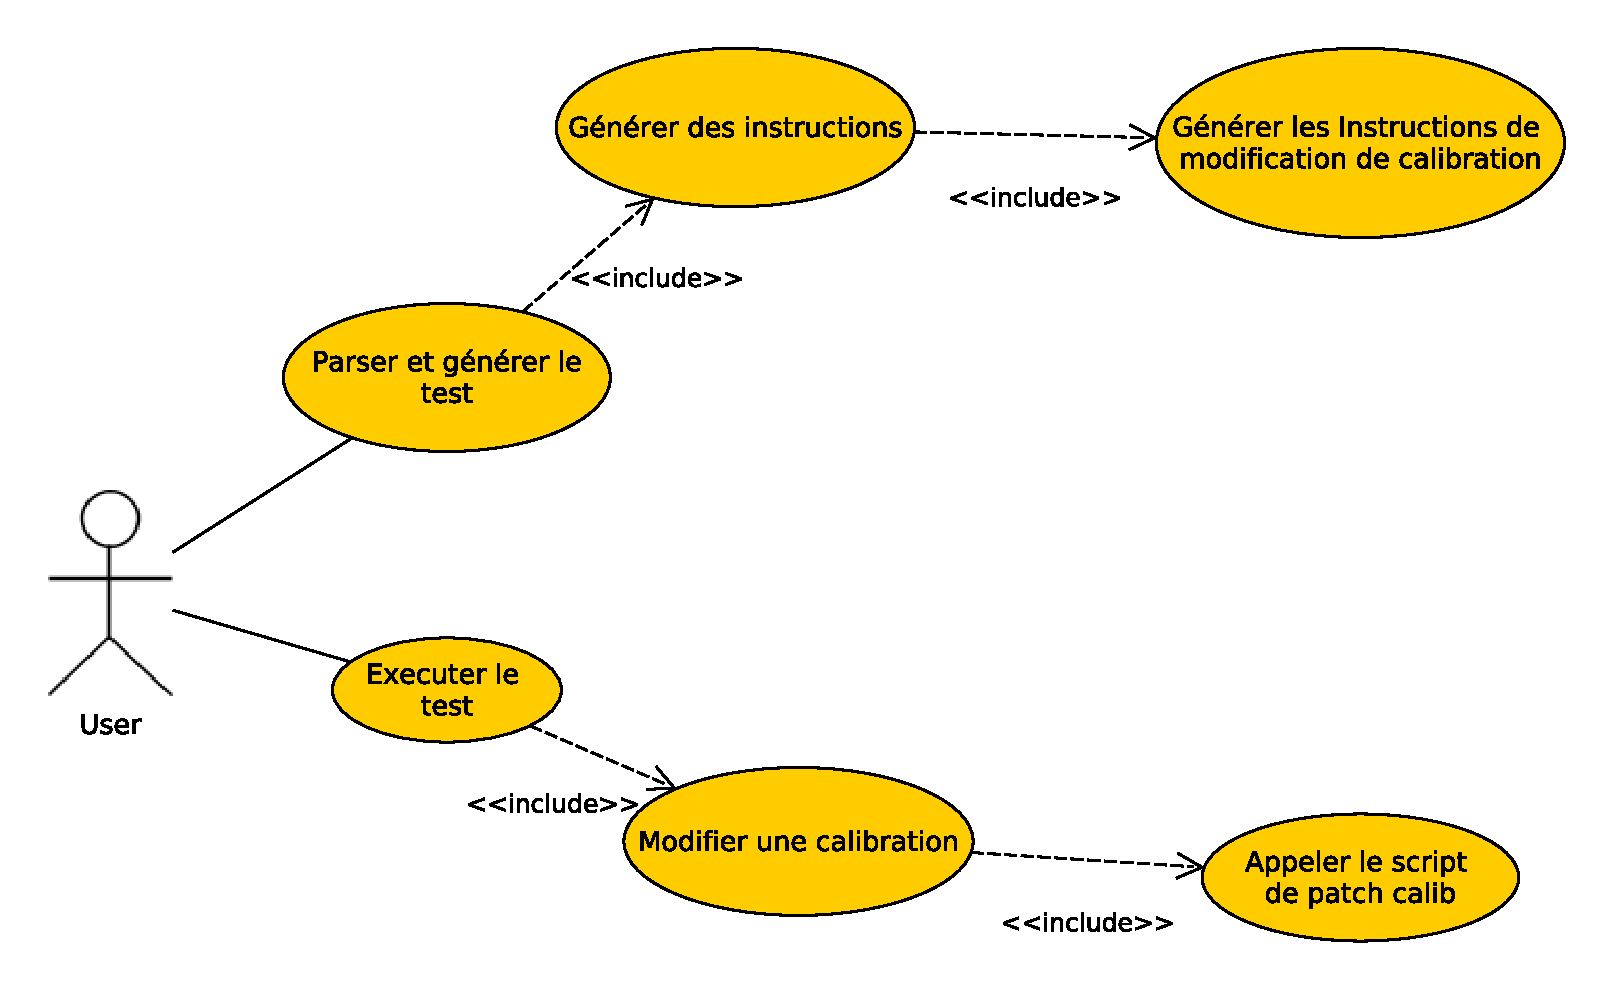
\includegraphics[width=18cm]{contents/images/patch-cal_usecase.eps}
			\caption{Diagramme de cas d'utilisations du patch de calibrations}
			\label{fig:patch-cal-usecase}
		\end{figure}

		\subsubsection{Limitations du \textit{patch calib}}
		Afin de concevoir au mieux la solution répondant aux besoins du client, j'ai tout d'abord du me renseigner sur la manière dont je pouvais effectuer cette action sur l'ECU, c'est-à-dire l'implémentation du serveur. Après discussions avec les personnes compétentes, une restriction impactant mon développement a été mis au clair.
		
		Afin de modifier une calibration, il est nécessaire de modifier la mémoire flash. Cette modification va nous obliger à éteindre l'ECU, la modification de la flash étant impossible ECU on. Il ne sera donc pas possible de modifier une calibration au milieu d'un scénario de stimulation, le scénario n'aurait aucun sens si nous éteignons et rallumons l'ECU pendant celui-ci.
		
		Cette restriction n'a cependant pas d'impact sur les tests qui seront rédigés, un scénario de stimulation a pour but de se rapprocher du fonctionnement nominal d'une voiture, or il est inconcevable de modifier une calibration pendant que la voiture tourne. Du point de vue des tests, ce choix reste cohérent. 
		
	\subsection{Utilisation de la fonctionnalité}\label{usePatch}
	%% Bla bla bla ici utilisation truc déjà rédigé
	
	\subsection{Conception et développement}
	Nous avons vu dans la section \ref{besoin-patch} que la fonctionnalité était répartie en deux grandes parties, le parser et l'exécution. Ces deux parties peuvent également s'apparenter à deux modules bien distincts de \textit{GreenT} : le client, pour le parser, et le serveur Debugger, pour l'exécution. Dans la suite de ce document, nous feront abstraction de l'utilisation de Thrift pour la communication réseau, celle-ci étant généré comme expliqué section TODO SECTION TOOLS.
	
	\subsubsection{Le serveur T32 : Exécution}
		\begin{wrapfigure}{r}{5.5cm}
			\vspace{-30px}
			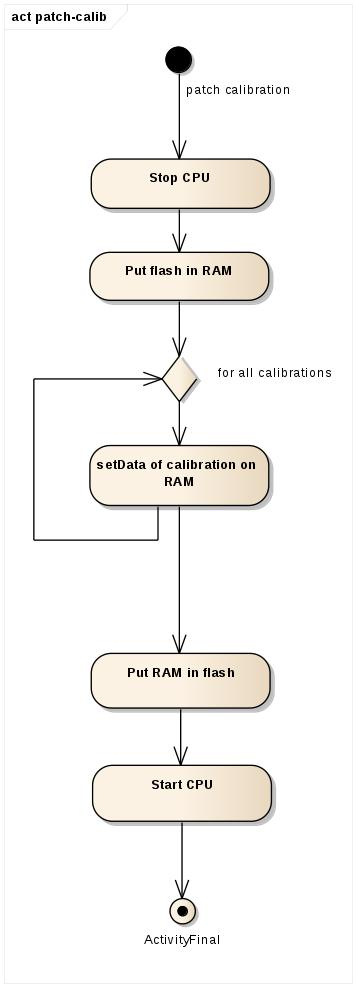
\includegraphics[height=17cm]{contents/images/script_activite.jpg}
			\caption{Diagramme d'activité du patch calib}
			\label{fig:scriptBatch} 
						\vspace{-7cm}
		\end{wrapfigure}
	Comme expliqué section TODO REF, le serveur du debugger utilise l'outil Trace32. C'est cet outil qui nous permet d’interagir avec le calculateur embarqué. Cet outil possède fonctionne principalement en utilisant des scripts batch.\\
	Depuis l'interface de cet outil, il est possible de patcher une calibration comme le montre la figure TODO test.
	%
	% INSERER ICI UNE CAPTURE D'ÉCRAN

	\begin{description}
		\item[Le script existant] Ce script a été pensé pour le mode graphique. L'utilisateur appelle le script, modifie les valeurs des calibrations voulues via l'interface , et cliquait sur « patch calibration ». À ce moment là, le patch en flash s'effectuait.
		\item[Le nouveau script] Le nouveau script va effectuer les même actions que le script existant, mais sans aucune attente d'actions utilisateurs. Pour cela, plutôt que d'attendre que l'utilisateur modifies les calibrations, nous aurons une liste calibration à modifier.
	\end{description}

	Afin de modifier une calibration, présente en flash, un certain nombre d'actions sont nécessaires. Ces actions sont montrés dans le diagramme d'activité figure \ref{fig:scriptBatch}.
	
	Le service du serveur va ainsi appeler le nouveau script de patch, le code Java concerné sera donc minime. Le prototype de la méthode est la suivante : 
	\begin{lstlisting}[language=Java, numbers=none]
public void patchCalibs(Map<String, Long> calibs);
	\end{lstlisting}
\newpage
	\subsubsection{Le client : Parser \& générateur}
	Afin de gérer le parsing et la génération de notre patch calib, j'ai du créer une nouvelle règle de grammaire comme montré section \ref{usePatch}. 
	
	Avec cette nouvelle grammaire, j'ai forcé l'utilisateur à ne modifier des calibrations que si l'ECU est éteint, cette action n'étant possible que dans une \texttt{patch section}. Une fois la liste de calibration à patchée parsée, il m'a suffit de générer l'instruction d'appel du Debugger.
	
	\begin{lstlisting}[language=Java]
Map<String, Long> calibrations = new HashMap<String, Long>();
calibrations.put("calib1", 0x0);
calibrations.put("calib2", 0x1);
dbg.patchCalibs(calibrations);
// Stimulation instructions
	\end{lstlisting}
	
	Cependant, afin de répondre à un besoin de l'équipe cliente, j'ai ajouté une sauvegarde de la valeur des calibrations avant le premier scénario, et une restauration à la fin du dernier scenario. Ceci pour garantir une bonne cohérence, en effet, si l'utilisateur modifie une calibration, celle-ci doit être à la bonne valeur pour les tests suivants. Cette restauration se fait de façon implicite afin de limiter le travail des testeurs, qui pourrait être source d'erreur.
	
	\subsection{Les difficultés rencontrées}
	\subsubsection{La robustesse}
	\subsubsection{Le batch}
\section{Les << tableaux calibrables >>}
	\subsection{Expression du besoin}
		\subsubsection{Cas d'utilisations}
		\subsubsection{Limitations des tableaux calibrables}
	\subsection{Conception et développement}

% <<< HEAD
% =================================================================================================
\section{La maintenance}
Comme expliqué plus haut, j'ai développé deux fonctionnalités durant ce stage. Cependant, en parallèle de ce développement j'ai également corrigés différents bugs, ou améliorer différentes partie de la plateforme.

Ayant conçu cette plateforme lors de mon stage de fin de Licence, je connais l'intégralité de la plateforme; C'est ainsi que j'ai pu détecter et corriger un certains nombres de problèmes. Ces bugs ou ces améliorations ont été identifiées de trois façons différentes : 
\begin{itemize}
	\item Durant mon développement, il m'est arrivé de trouver du code incohérent ou bouchonné
	\item Lors d'exécutions de la plateforme sur différentes versions du projet client
	\item En regardant les différents tickets ouverts et devant être résolus
\end{itemize}

\subsection{Corrections}
J'ai corrigé quelques problèmes trouvés sur la plateforme, principalement venant du client \textit{GreenT}. Ceci étant dû à notre choix d'architecture : des serveurs les plus légers et un client effectuant le maximum d'actions.
	\subsubsection{Stockage des erreurs d'exécutions}
	\begin{description}
		\item[Le problème] En cas d'erreur durant une exécution, si un serveur ne répond plus, si une variable est non trouvée, ... Une exception est levée. À ce moment là, \textit{GreenT} doit attraper l'exception et la stocker en base de données pour pouvoir afficher ensuite le message à tous les tests du bundle, la génération des rapports ne pouvant pas se faire.
		\item[La solution] Le stockage du message d'erreur n'était pas fait, ainsi que la requête SQL permettant d'obtenir les messages d'erreurs. Ces deux actions ont été corrigés, en lieu et place du rapport de test nous avons maintenant un message d'erreur clair.
		\end{description}
		
	\subsubsection{Modification des variables Debugger}
		\begin{description}
			\item[Le problème] Lors d'un stimulus, il est possible de modifier une variable Debugger. Lors de la modification d'une variable, le Trace32 renvoyait toujours une exception, sans appliquer la modification.
			\item[La solution] Après lecture de la documentation de Trace32, il s'est avéré que le problème venait simplement du serveur qui appliquait une commande syntaxiquement incorrecte. La modification de la commande a corrigée le problème.
	\end{description}
	
	\subsubsection{Ordre d'exécutions des scénarios}
		\begin{description}
			\item[Le problème] Un Test peut contenir plusieurs scénarios, ceux-ci nous servent principalement pour le << patch-calib >> comme expliqué section \ref{patch}. Or, si nous utilisions plusieurs scénarios, ceux-ci étaient exécutés dans un ordre aléatoire : si l'utilisateur voulait effectuer des actions dans un ordre donnée, ce n'était pas possible.
			\item[La solution] Le problème avait deux parties : d'une part, l'exécution des scénarios dans un ordre donné, d'autre part, spécifier un ordre à chacun de nos scénarios. En effet, tout d'abord, j'ai nommé les scénarios de sortes qu'ils soient classé par ordre alphabétique. Ensuite, il a fallu spécifier à la plateforme d'exécuter les différents scénarios dans un ordre alphabétique, pour cela il a suffit d'utiliser une collection Java effectuant cette action, la \texttt{TreeMap}.
	\end{description}
	
	\subsubsection{Reset ECU à l'exécution}
	\begin{description}
		\item[Le problème] Lors de l'exécution de notre plateforme sur la dernière version du projet client, nous avions systématiquement un \textit{reset} ECU. C'est-à-dire que notre ECU s'arrêtait et ne redémarrait pas pour une raison inconnue.
		\item[La solution] Le problème ne venait pas directement de la plateforme, mais d'une mauvais configuration de notre part. En effet, nous ne spécifions pas les bons fichiers du logiciel, celui-ci étant mal flashé, l'ECU refusait de démarrer.
	\end{description}
	
	\subsubsection{Absence d'injection}
	\begin{description}
		\item[Le problème] Lorsque j'essayais de simuler un démarrage du moteur sur la dernière version du logiciel, aucune injection ne se faisait : après le starter, le moteur retournait à 0 tour.
		\item[La solution] Après s'être renseigné auprès de personnes compétentes, il s'est avéré que cela venait d'un nouveau fichier à flasher dont nous n'avions pas connaissance. Un fichier contenant des calibrations permettant le démarrage du moteur sur table. Ce fichier n'ayant pas été pris en compte durant la conception, j'ai ajouté un nouveau paramètre au fichier de configuration permettant de renseigner des fichiers à flasher additionnels.
	\end{description}
	
\subsection{Améliorations}
	\subsubsection{Exécution différée} %
	\begin{description}
		\item[Le besoin] Lors de mon développement, j'ai eu souvent des problèmes pour réservés des tables de tests. Celles-ci étant régulièrement prise par les équipes projets. 
		\item[La solution] Afin de ne pas bloquer de tables, et de ne pas bloquer notre travail en raison de l'absence de celles-ci, une solution nous est venue : la possibilité de lancer l'outil durant la nuit. En effet, actuellement une exécution dure environ 45 minutes, après laquelle nous pouvons analyser les rapports et voir les problèmes qui nous sont retournés. Ainsi, j'ai ajouté un nouveau paramètre à l'application permettant de spécifier à laquelle la génération, la compilation, l'exécution et la génération des rapports va se faire. On peut maintenant lancer une exécution le soir et observer les résultats le lendemain matin.
	\end{description}
	
	\subsubsection{Passage à Java 8}
		\begin{description}
			\item[Le besoin] La plateforme fonctionnait sous Java 6. Ainsi, nous allions mettre en production une plateforme déjà obsolète à sa sortie. De plus, les deux versions suivantes de Java propose un certain nombre de fonctionnalité aidant au développement, comme des simplifications d'écriture en Java 7 (\textit{Multi-Catch}, Inférence de type, \texttt{switch} sur les strings, ...) ou les lambdas-calculs en Java 8. Enfin, dans un future proche nous aurons besoin d'une interface pour \textit{GreenT}, \textit{JavaFx} serait une bonne solutions, mais celle-ci nécessite Java 8.
			\item[La solution] Avant de passer à Java 8, il a d'abord fallut vérifier qu'aucune incompatibilité avec les bibliothèques que nous utilisons n'allait apparaître. Ensuite, il était nécessaire de télécharger un compilateur ainsi qu'une JVM, configurer les différents environnements et vérifier qu'une exécution se passait de la même manière que précédemment. Après ce succès, le passage à Java 8 a été concrétisé et permet à notre plateforme de rester moderne ! 
		\end{description}
		
	\subsubsection{<< \textit{Clean-Code} >>}
		\begin{description}
			\item[Le besoin] \textit{GreenT} ayant deux ans, et ayant connue 4 développeurs différents, il est parfois nécessaire d'améliorer le code existant ou de le rendre plus lisible. 
			\item[La solution] Lorsqu'en développant mes fonctionnalités ou en corrigeant des bugs je tombais sur du code incompréhensible ou du << code mort >>, je modifiais celui-ci afin de corriger ces défauts. Ceci permet ainsi de garder un code toujours propre et facile à lire.
		\end{description}
		
	\subsubsection{Affichage des \textit{logs}}
		\begin{description}
			\item[Le besoin] La plateforme effectue beaucoup d'actions, allant du parsing jusqu'à la génération des rapports comme montré chapitre \ref{chapGreent}. Toutes ces actions doivent être tracés, aussi bien en tant réel, en regardant l'exécution que plus tard en observant un fichier.
			\item[La solution] Les logs fonctionnait déjà, en utilisant \texttt{log4j}, cependant celui-ci affichait beaucoup trop d'informations en temps réel, et n'affichait pas les informations les plus utiles. Ainsi, j'ai passé en revue la plateforme pour afficher les bonnes actions (Initialisation des bancs, stimulis effectués, affichage des exceptions, \ldots). Toutes les erreurs sont redirigé vers la sortie des erreurs (\texttt{stderr}), et seules les informations les plus importantes sont sur la sortie console (\texttt{stdout}). Tous les autres logs, qui peuvent être utile à la compréhension d'un problème et nous aider ne sont accessible que dans nos fichiers de logs. J'ai par ailleurs ajouté un « buffer tournant » permettant aux fichiers de logs de ne jamais dépasser une certaines taille (5Mio), afin de ne pas consommer trop d'espace.
		\end{description}
		

